\chapter{Approche Théorique}
\section{Introduction}

In this chapter we will start by presenting the used paradigms and approaches, the global domain Diagram used in the analysis phase. And then we will explain the different components and their behavior.

\section{Formalisation}\cite{4}
Le BNN, bien que son objectif est clair, elle n'a pas d'approche triviale pour arriver à un réseau "binaire". Pour cela, on va tout d'abord formaliser notre objectif, est après ça, on va essayer de définir un BNN

\subsection{Notations}
Pour simplifier, nous allons commencer par la terminologie des réseaux à perceptrons multicouches.
\pagebreak
\subsubsection{Observations}\label{Theoretical:Observations}
\begin{table}[ht]
	\centering
	\begin{tabularx}{\textwidth}{| X | X |}
		\hline
		$r$ & nombre d'exemplaires du jeux de données \\ 
		\hline
		$\boldsymbol{X}^{\{k\}}$ & l'entrée du $k^\text{ème}$ exemplaire \\
		\hline
		$\boldsymbol{X}=\left(\boldsymbol{X}^{\{1\}},\dots, \boldsymbol{X}^{\{r\}}\right)$ & le tenseur des entrées \\
		\hline
		$\boldsymbol{Y}=\left(\boldsymbol{Y}^{\{1\}},\dots, \boldsymbol{Y}^{\{r\}}\right)$ & le tenseur des résultats \\
		\hline
		$\boldsymbol{U}=\left(\boldsymbol{U}^{\{1\}},\dots, \boldsymbol{U}^{\{r\}}\right)$ & le tenseur des observations \\
		\hline
		
		$\hat{\boldsymbol{Y}}$                    & Une estimation de $\boldsymbol{Y}$      \\ 
		\hline 
		$\mathcal{L}$                    & Une fonction objective      \\ 
		\hline 
		$\mathcal{L}(\hat{\boldsymbol{Y}},\boldsymbol{Y})$                    & L'erreur d'estimation de $Y$       \\ 
		\hline 
	\end{tabularx}
	\caption{Terminologie des jeux de données}
	\label{table:Datasets}

\end{table}

\subsubsection{Division en Lots}
\begin{table}[ht]
	\centering
	\begin{tabularx}{\textwidth}{| X | X |}
		\hline
		$m$ & nombre de lots \\ 
		\hline
		$s_k$ & la taille du $k^\text{ème}$ lot \\
		\hline
		$\boldsymbol{X}^{[k]}$ & le $k^\text{ème}$ lot d'entrées \\
		\hline
		$\boldsymbol{Y}^{[k]}$ & le $k^\text{ème}$ lot de sorties \\
		\hline
		$\boldsymbol{U}^{[k]}$ & le $k^\text{ème}$ lot des observation \\ 
		\hline
		
		$\mathcal{L}(\hat{\boldsymbol{Y}}^{[k]},\boldsymbol{Y}^{[k]})$                    & l'erreur d'estimation de $k^\text{ème}$ lot       \\ 
		\hline 
		
	\end{tabularx}
	\caption{Terminologie de la division en Lots}
	\label{table:Batch}
\end{table}
\begin{remark}
	Par défaut, on va diviser les lots en une taille fixe $s$. \newline
	Comme une exception, le dernier lot va avoir le reste de cette division
\end{remark}
\FloatBarrier
\newpage

\subsubsection{MLP et CNN}
\begin{table}[ht]
	\centering
	\begin{tabularx}{\textwidth}{| X | X |}
		
		\hline
		$\mathcal{N}$          & Un réseau de neurones \\ 
		\hline
		$\mathcal{N}_{\boldsymbol{W}}$          & Un réseau de neurones définit par le tenseur $\boldsymbol{W}$      \\ \hline
		$\boldsymbol{W}^{(l)}$          & La matrice de liaison de la $l^\text{ème}$ couche         \\
		\hline
		$\sigma^{(l)}$& la fonction d'activation de la $l^\text{ème}$ couche \\
				\hline
		$z^{(l)}=\boldsymbol{W}^{(l)}\star a^{(l-1)}$ & le contenu de la couche $l$ avant l'activation\\
		\hline
		$a^{(l)}=\sigma^{(l)}({z^{(l)}})=\sigma^{(l)}(\boldsymbol{W}^{(l)}\star a^{(l-1)})$ & le contenu de la couche $l$ après l'activation \\
		\hline
		$W^{(l)}_{i,j}$                 & le poids de neurone $a^{(l-1)}_{j}$ dans la $i^\text{ème}$ neurones avant l'activation           \\ \hline
		$x=a^{(0)}$                    & L'entrée du réseau de neurones          \\ \hline
		$\hat{y}=a^{(l)}=\mathcal{N}_{\boldsymbol{W}}(x)$              & La sortie du réseau de neurones  \\ \hline
		$n_l$ & le nombre de neurones de la $l^\text{ème}$ couche \\ 
		 \hline 
		
	\end{tabularx}
	\caption{Different machines characteristics}
	\label{table:AcyclicNeuralNetwork}
	\begin{remark}
		Le terme $W^{(l)} \star a^{(l-1)}$ est  interprété comme:
		\begin{enumerate}
			\item une multiplication matricielle $W^{(l)}\cdot a^{(l-1)}$ dans le cas d'une couche dense
			\item une opération de convolution $W^{(l)}* a^{(l-1)}$ dans le cas d'une couche convolutionelle
		\end{enumerate}
		 
	\end{remark}
\end{table}
\FloatBarrier


\subsection{Définition d'un BNN}
Avant de définir un BNN, nous allons introduire le concept des binarisations et des quantifications:
\begin{definition}
	Une binarisation est une fonction $\Psi:\mathbb{R}\rightarrow \mathcal{B}$ avec $\mathcal{B}$ un ensemble à deux éléments.
	\newline Dans le cas d'un tenseur, la binarisation est appliquée élément par élément.
	\newline On va distinguer essentiellement deux valeurs particulières de $\mathcal{B}:$
	\begin{itemize}
		\item $\mathcal{B}=\{\pm 1\}$
		\item $\mathcal{B}=\{0,1\}$
	\end{itemize}
\end{definition}
\begin{definition}
	Un scalaire $u$ est dit binarisé s'il varie dans un ensemble $\mathcal{B}$ à deux éléments.
	\newline Un tenseur de rang $r$ et de dimension $n_1\times\dots\times n_r$ est dit binarisé s'il varie dans un ensemble $\mathcal{B}^{n_1\times\dots\times n_r}$ avec $\mathcal{B}$ à deux éléments.
\end{definition}
\begin{definition}
	Une quantification est un opérateur $\Psi$ appliqué à un tenseur juste avant l'opération bilinéaire en conservant ses dimensions.
\end{definition}
\begin{remark}
	Dans les réseaux de neurones classiques, il n'y a pas de quantifications. En faite, l'absense d'une quantification est équivalente à l'utilisation de la quantification $\mathtt{id}:x\rightarrow x$
\end{remark}

\subsubsection{Dans la littérature}
Le BNN n'admet pas d'une définition unique. En contre partie, dans la littérature\cite{BNNDefinition}, la plupart des réseaux sont nommées binaires puisque :
\begin{enumerate}
	\item Pour chaque paire de nœuds connexe $(u,v).$ Le poids de la liaison est $\omega(u,v)=\pm 1$
	\item Pour chaque couche cachée, la fonction d'activation est la fonction signe $\sign$
\end{enumerate}
\subsubsection{Notre définition}
Nous avons proposé cette définition pour essaier d'unifier les approches des BNNs:
\begin{definition}
Un BNN est tout réseau de neurones admettant au moins une couche dont les quantifications sont des binarisations
\newline Un BNN idéal est un réseau de neurones dont toutes les quantifications sont des binarisations
\end{definition}
\begin{remark}
	Dans ce stage, nous allons concentrer sur les binarisations dont $\mathcal{B}=\{\pm 1\},$ et surtout la binarisation $\sign$
\end{remark}
\begin{remark}
	Bien que la définition est un peu permissive, nous n'allons considérer que les BNNs qui on un nombre "important"\footnote{Grosso modo, le nombre de binarisations doit être aussi important pour justifier les apports des binarisations.} de binarisations.
\end{remark}
\subsection{Objectif}
\subsubsection{Notations}
\begin{itemize}
\item Soit $\mathcal{D}=\left(\boldsymbol{X},\boldsymbol{Y}\right)$ le jeu de données
\item Soit $\mathcal{N}_{\boldsymbol{W}}$ un réseau de neurones admettant le tenseur de paramètres $\boldsymbol{W}.$ 
\end{itemize}
\subsubsection{Problème d'optimisation}
 L'objectif "idéal" est la résolution du problème d'optimisation suivant:
\begin{equation}\label{ObjectiveFunction}
	\boldsymbol{W}^*=\argmin_{\boldsymbol{W}} \mathcal{L}\left(\mathcal{N}_{\boldsymbol{W}}(\boldsymbol{X}),\boldsymbol{Y}\right)
\end{equation}
L'objectif pour un BNN est aussi la minimisation de \eqref{ObjectiveFunction}, mais la seule différence est que le réseau admet des binarisations comme quantifications.
\newpage


\section{Entraînement}

Notre définition de BNN pose beaucoup de problème dans l'entraînement, dont la résolution exige des approches sophistiquées.

\subsection{Difficulté du problème discret}
Soit $\mathcal{N}$ un réseau de neurones binaire idéal ayant une topologie fixe, et soit $\eta$ le nombre total de ses paramètres binarisés. 
\newline Dans le plus mauvais cas, la complexité de trouver les valeurs optimales des paramètres pour ce réseau est  $\mathcal{O}(2^\eta)$ qui n'est pas du tout pratique.

Deux solutions se présentent:
\begin{enumerate}
	\item Approcher le problème discret avec des algorithmes d'approximations et des heuristiques.
	\item Retourner à l'optimisation continue de la fonction objective, 
\end{enumerate}


\subsection{Gradient Nul}
Nous allons opter pour la deuxième solution dans ce stage. Mais, malheureusement, on ne peut pas appliquer directement les méthodes d'optimisations de premier ordre, ou même d'ordre supérieur.
\newline Le problème majeur provient de la lemme suivante:
 \begin{lemma}
 	Toute binarisation continue presque partout\footnote{Le mot "presque partout" est interpreté au sens de la théorie des mesures, et précisément la mesure naturelle dans $\mathbb{R}$ (mesure de Leibniz). Par exemple, dans un sens, la "dérivée" de la fonction $\sign$ est la fonction de Dirac $\delta$} admet une dérivée nulle presque partout
 \end{lemma}
\begin{proof}
	Soit $\Phi:\mathbb{R}\rightarrow \{a_0,a_1\}$ une binarisation continue partout sauf un ensemble $\mathcal{D}$ de mesure nulle, avec $a_0,a_1\in\mathbb{R}$ et $a_0\neq a_1.$
	\newline Soit $x_0\in\mathbb{R}$ tels que $\Phi$ est continue en $x_0,$ et soit $0 <\epsilon < \lvert a_1 -a_0 \rvert$ et $\delta\in\mathbb{R}_+^*$ tel que $$x\in\mathscr{B}(x_0,\delta)\implies \lvert \Phi(x)- \Phi(x_0)\rvert < \epsilon$$
	On a nécessairement, $\Phi(\mathscr{B}(x_0,\epsilon))= \{a_i\}$ avec $i\in\{0,1\}$, et donc $\Phi$ est constante sur $\mathscr{B}(x_0,\delta),$ et ainsi dérivable sur cet interval et en particulier en $x_0$, et on a: 
	$$
	\Phi'(x_0)=0
	$$
	Ainsi:
	$$
	\forall x\in\mathbb{R},\quad \Phi \ \text{continue en} \ x \implies \Phi \ \text{dérivable en} \ x \ \text{et}\ \Phi'(x)=0  
	$$
	Finalement, on a $\Phi$ est continue sur $\mathcal{S}=\mathbb{R}\setminus\mathcal{D}$, avec $\mathcal{D}$ est de mesure nulle, et donc $\Phi$ est dérivable sur $\mathcal{S}$  et par conséquent $\Phi'=0$ sur $\mathcal{S} \ \blacksquare$
\end{proof}
Cette lemme pause un problème puisque la mise à jour des paramètres sera impossible avec des gradient nuls presque partout.
\newline 
Pour résoudre ce problème, nous pouvons:
\begin{enumerate}
	\item Faire une approximation de la binarisation par une fonction plus régulière, surtout dans la propagation en arrière.
	\item Faire une relaxation concernant la notion de gradient à l'aide d'un opérateur $\mathcal{G}$ adéquat "avec lequel on peut appliquer les méthodes de premier ordre.
\end{enumerate} 
Dans le chapitre suivant, nous allons voir chacune des approches 1 et 2.
\begin{figure}[htp!]
	\centering
	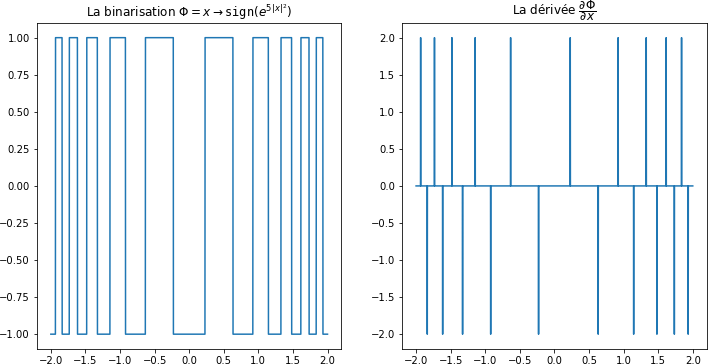
\includegraphics[width=.75\textwidth]{Figures/binarisation-plot.png}
	\caption{Un exemple d'une binarisation et sa dérivée}
	\label{fig:Binarisation-Example}
\end{figure}
\FloatBarrier
\newpage
\section{Optimisations}
\subsection{Définitions}
On note par:

\begin{itemize}
\item $(\mathbb{B},+,\cdot,\bar{},0,1 )$ une algèbre de boole.
\item l'opérateur $\mathtt{XOR}$ par $\oplus$ défini par:
\newline $a\oplus b = \mathtt{XOR}(a,b)=a\cdot \bar{b}+\bar{a}\cdot b=\bar{a}\oplus \bar{b}$
\item l'opérateur $\mathtt{XNOR}$ par $\odot$ défini par:
\newline $a\odot b = \mathtt{XNOR}(a,b)=\overbar{\mathtt{XOR}(a,b)}= (a + \bar{b}) (\bar{a}+b) = a\cdot b + \bar{a} \cdot \bar{b}=\bar{a}\odot \bar{b}$
\end{itemize}

\subsection{Codage sur $1\text{bit}$}
Puisque les poids et noeuds des couches cachées sont tous binarisés, on peut coder chaque valeur sur un seul bit. Ainsi on peut introduire le codage: 
$$\Psi: \begin{cases}
	-1 & \rightarrow 0 \\
	1 & \rightarrow 1
\end{cases}$$

En faite, on regroupe chaque $8$ variables dans la même case mémoire.

\subsection{Utilisation de $\mathtt{XNOR}$}
\subsubsection{Transformation de $\times$ en $\mathtt{XNOR}$}
Dans le cas d'un BNN, les noeuds et les poids sont binarisés. Ainsi toute multiplication est entre deux éléments de $\{-1,1\}.$
\newline Or, par la transformation bijective: 
$$\Psi:\begin{cases}
	1 &\rightarrow 1 \\
	-1 &\rightarrow 0
	\end{cases}$$
On a l'égalité suivante:
$$
\forall a,b\in\{-1,1\},\quad \Psi(a\times b) = \Psi(a)\odot \Psi(b) 
$$
\begin{figure}[h!]
	\centering
	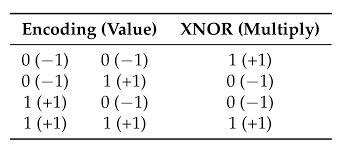
\includegraphics[width=.5\textwidth]{Figures/XNOR-Table.png}
	\caption{Table de multiplication en utilisant XNOR}
	\label{fig:XNOR-Table}
\end{figure}
\FloatBarrier
\begin{proof}
	On a le groupe $(\mathbb{C}_2,\times )$  avec $\mathbb{C}_2=\{z\in \mathbb{C} / \quad z^2=1\}=\{-1,1\}$ est cyclique et d'ordre $2.$ Ainsi, il est isomorphe au groupe $(\mathbb{F}_2,\oplus)$ où $\mathbb{F}_2=\mathbb{Z}/2\mathbb{Z}=\{0,1\},$ et $\oplus$ est l'addition modulo $2$. 
	\newline L'ismorphisme entre eux est: 
	$$\Psi_1=\begin{cases}
		-1 & \rightarrow 1 \\
		1 & \rightarrow 0
	\end{cases}$$
	De plus, le corps $(\mathbb{F}_2,\oplus,\times)$ induit l'algèbre de boole $(\mathbb{F}_2,+,\times,\bar{},0,1)$ avec:
	\begin{align*}
		\bar{a}&=a\oplus 1 \\
		a+ b &= \overbar{\bar{a}\times\bar{b}}
	\end{align*}
	Or, par dualité de l'algèbre booléenne, l'opérateur de négation $\Psi_2:a\rightarrow \bar{a}$ est un isomorphisme entre $(\mathbb{F}_2,+,\times,\bar{},0,1)$ et $(\mathbb{F}_2,\times,+,\bar{},1,0)$
	
	Ainsi on a:
	\begin{align*}
	\forall a,b\in\{-1,1\}, \quad \Psi_2\circ \Psi_1( a\times b)  &= \Psi_2(\Psi_1(a\times b)) \\
			&=\Psi_2(\Psi_1(a)\oplus \Psi_1(b)) \ \text{isomorphisme 1} \\ 
			&=\overbar{\Psi_1(a)\oplus \Psi_1(b)}  \\
			&=\Psi_1 (a) \odot \Psi_1(b) \ \text{isomorphisme 2} \\
			&= \overbar{\Psi_1 (a)} \odot \overbar{\Psi_1(b)} \\
			&= \Psi_2\circ \Psi_1 (a) \odot \Psi_2\circ \Psi_1(b)  
	\end{align*}
	Maintenant, il ne reste qu'à vérifier que $\Psi=\Psi_2\circ \Psi_1:$
	\begin{align*}
		\Psi_2\circ \Psi_1(-1) &=\Psi_2(\Psi_1(-1))\\
		&=\Psi_2(1) \\
		&=0 \\
		\Psi_2\circ \Psi_1(1) &=\Psi_2(\Psi_1(1))\\
		&=\Psi_2(0) \\
		&=1 \quad \blacksquare
	\end{align*}
\end{proof}
\subsubsection{Avantages}
En faite, dans les circuits intégrés, l'opération $\mathtt{XNOR}$ est plus rapide que $\times$. En faite, elle:
\begin{itemize}
	\item consomme moins d'énergie
	\item peut être faite $32$ fois dans un seul cycle. Par comparaison, une seule opération $\times$ peut dépasser $1$ cycle 
\end{itemize}
 \newpage
\subsection{Utilisation de $\mathtt{POPCOUNT}$}
	\subsubsection{Définition de $\mathtt{POPCOUNT}$}
	$\mathtt{POPCOUNT}$ est une instruction qui permet de compter les bits qui sont mis à $1$ dans un vecteur de bits $v.$
	\begin{remark}
		$v$ peut être la représentation binaire d'un nombre $n$
	\end{remark} 
	\subsubsection{Produit scalaire de deux vecteurs binarisés}
	Soit $u,v\in\{-1,1\}^n.$ On a:
	\begin{align*}
		\langle u,v \rangle &=\sum_{i=1}^n u_iv_i \\ 
		&=  \sum_{i=1}^n \Psi^{-1}(\Psi(u_i)\odot\Psi (v_i)) \\
		&= \mathtt{POPCOUNT}(\Psi(u)\odot \Psi(v)) \cdot \Psi^{-1}(1) + \left(n-\mathtt{POPCOUNT}(\Psi(u)\odot \Psi(v))\right)\cdot \Psi^{-1}(0) \\
		&= \mathtt{POPCOUNT}(\Psi(u)\odot \Psi(v))-\left(n-\mathtt{POPCOUNT}\left(\Psi(u)\odot \Psi(v)\right)\right) \\
		&= 2\cdot \mathtt{POPCOUNT}(\Psi(u)\odot \Psi(v)) - n \\
		&= \left(\mathtt{POPCOUNT}\left(\Psi(u)\odot \Psi(v)\right) \ll 1 \right) - n
	\end{align*}
	\begin{figure}[h!]
		\centering
		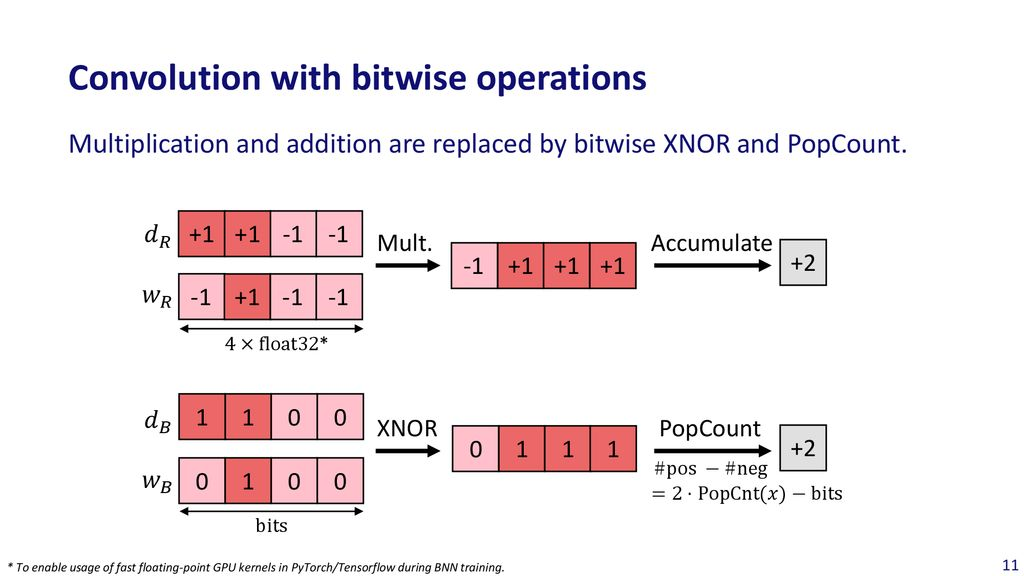
\includegraphics[width=.9\textwidth]{Figures/POPCOUNT.jpg}
		\caption{Calcul du produit scalaires}
		\label{fig:POPCOUNT}
	\end{figure}
\pagebreak
	\subsubsection{Estimation de coût}
	 On suppose pour $m\in \mathbb{N}^*$, que notre processeur supporte dans une seule instruction, un $\mathtt{XNOR}$ bit-wise des deux vecteurs bits $u,v\in\{0,1\}^m$  
	\newline On suppose aussi pour cette même valeur de $m$ que notre processeur supporte dans une seule instruction, un $\mathtt{POPCOUNT}$ bit-wise d'un vecteur bits $u\in\{0,1\}^m$  
	\newline Soit $n=mr, \ r\in\mathbb{N}^*,$ et soit $u,v\in\{-1,1\}^n$ 
	\newline Pour $p\in\{1,r\},$ soit: 
	$$\begin{cases}
		u^{[p]}=(u_{(p-1)m+1},\dots u_{pm}) \\ v^{[p]}=(v_{(p-1)m+1},\dots v_{pm})
		\end{cases}$$
	On a:
	\begin{align*}
		\langle u ,v\rangle &= \sum_{i=1}^{n} u_iv_i\\
		&= \sum_{p=1}^r \langle u^{[p]},v^{[p]}  \rangle \\
		&= \sum_{p=1}^r 2\cdot \mathtt{POPCOUNT}\left(\Psi\left(u^{[p]}\right) \odot \Psi\left(v^{[p]}\right)\right) - m \\
		&= 2\sum_{p=1}^r  \mathtt{POPCOUNT}\left(\Psi\left(u^{[p]}\right) \odot \Psi\left(v^{[p]}\right)\right) - \sum_{p=1}^r m \\
		&= \left( \sum_{p=1}^r  \mathtt{POPCOUNT}\left(\Psi\left(u^{[p]}\right) \odot \Psi\left(v^{[p]}\right)\right)  \ll 1\right)-n
	\end{align*}

	Ainsi, on a optimisé $n$ multiplications et $n-1$ additions en:
	\begin{itemize}
		\item $r-1=\frac{n}{m}-1$ additions.
		\item $r$ instructions $\mathtt{XNOR}$
		\item $1$ décalage à gauche.
		\item $1$ soustraction.
	\end{itemize} 
\pagebreak
\subsection{Gain Temps \& Mémoire}
\subsubsection{Gain Mémoire}
Les implémentations classiques des RN utilisent des paramètres en firgules flottantes à precision simple. c'est à dire chaque paramètre prends $32 \ \text{bits}.$
\newline Avec le codage considéré, on peut avoir un gain de mémoire $\alpha_{\text{mémoire}}=32$

\subsubsection{Gain Temps}
Le gain de l'opération de produit scalaire est:
\begin{align*}
\alpha_{\langle \cdot , \cdot \rangle} &= \frac{n+n-1}{\frac{n}{m}-1+\frac{n}{m}+1+1}  \\
&= \frac{2n-1}{2\frac{n}{m}+1} \\
&= \frac{2-\frac{1}{n}}{2\frac{1}{m}+\frac{1}{n}} \\
&= \frac{2m-\frac{m}{n}}{2+\frac{m}{n}} \\
&= \frac{m-\frac{m}{2n}}{1+\frac{m}{2n}}\\
&= m -\frac{m(m+1)}{2n} + o\left(\frac{m^3}{n^2}\right)
\end{align*}

On a:
\begin{itemize}
	\item Pour un PC personnel, ou même téléphone: $m=64.$
	\item Pour les réseaux de neurones standards, $32\leq n\leq 1024$
\end{itemize}

Ainsi une estimation de $\alpha_{\text{temps}}$ est :
$$
31.5\leq \alpha_{\text{temps}} \leq \frac{2047}{32} \approx 62.03
$$